\newpage

\section{Fakultät}
Für alle natürlichen Zahlen n ist die Fakultät n! definiert als:\\ \\
$ n! = 1 * 2 * 3 * ... * n = \prod \limits_{i = 1}^{n}i$\\ \\
Beispiel:\\ \\
$6! = 6 * 5 * 4 * 3 * 2 * 1 = 720$ \\ \\

\section{Binomialkoeffizient}
Der Binomialkoeffizient $\binom{n}{k}$ ist definiert als:\\ \\
$\binom{n}{k} = \dfrac{n!}{(n - k)! * k!}$\\ \\
mit $0 \le k \le n,\quad k, n \in \mathbb{N}$.\\ \\
Beispiel:\\ \\
$\binom{5}{3} = \dfrac{5!}{(5 - 3)! * 3!} = \dfrac{5 * 4}{2!} = \dfrac{20}{2} = 10$\\ \\

\section{Bernsteinpolynome}
Die mathematische Grundlage zur Beschreibung von Bezier-Kurven geben die Bernsteinpolynome.\\ \\
Die Bernsteinpolynome (vom Grad n auf [0, 1]) sind definiert als:\\ \\
$B^{n}_{i}(t) = \binom{n}{i} * t^{i} * (1 - t)^{n - i}$\\ \\
mit $i = 0, ... , n, \quad n \in \mathbb{N}$\\ \\
Ein ihrer wichtigsten Eigenschaften ist dass sie die folgende Rekursionsformel erfüllen:
$B^{n}_{i}(t) = (1 - t)B^{n - 1}_{i}(t) + tB^{n - 1}_{i - 1}(t)$\\ \\
mit $B^{0}_{0}(t) \equiv{1}$ und $B^{n}_{j}(t) \equiv{0}$ für $j \notin {0, ... , n}$.\\ \\
Beweis:\\ \\
\begin{align*}
	B^{n}_{i}(t) &= \binom{n}{i}t^{i}(1 - t)^{n - i}\\
	&= \binom{n - 1}{i}t^{i}(1 -t)^{n - i} + \binom{n - 1}{i - 1}t^{i}(1 -t)^{n - i}\\
	&= (1 - t)B^{n - 1}_{i}(t) + tB^{n - 1}_{i - 1}(t)\\
\end{align*}
Eine andre wichtige Eigenschaft der Bernsteinpolynome ist, dass sie eine Teilung der Eins bilden:\\ \\
$\sum \limits_{j = 0}^{n}B^{n}_{j} \equiv{1}$\\ \\
Dies kann mit Hilfe des binomischen Satzes gezeigt werden:\\ \\
$1 = [t + (1 - t)]^{n} = \sum \limits_{j = 0}^{n}\binom{n}{j}t^{j}(1 - t)^{n - j} = \sum \limits_{j = 0}^{n}B^{n}_{j}(t)$\\ \\
\begin{figure}[h]
\centering
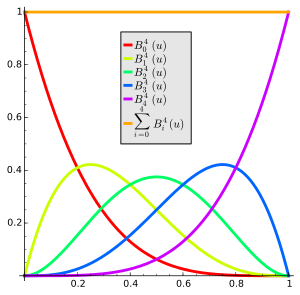
\includegraphics[width=0.5\linewidth]{images/Bernstein_Polynomials}
\caption{}
\label{fig:Bernstein_Polynomials}
\end{figure}
Abbildung 1 zeigt die Bernsteinpolynome $B^{4}_{i}, 0 \le i \le 4$ vom Grad 4 Man beachte, dass die $B^{n}_{i}}$ nicht negativ über dem Intervall [0, 1] sind.

\newpage	
\section{Quellen}
 \url{https://de.wikipedia.org/wiki/Fakult\%C3\%A4t\_(Mathematik)}